\chapter{Lowering the Cost of Compiler Validation}
\label{chap:deepsmith}


\section{Introduction}

Compilers should produce correct code for valid inputs, and meaningful errors for invalid inputs. Failure to do so hinders software development and even causes catastrophic runtime errors. Still, properly testing compilers is hard. Modern optimising compilers are large and complex programs, and their input space is huge. Hand-designed suites of test programs, while important, are inadequate for covering such a large space and will not touch all parts of the compiler.

Random test case generation --- \emph{fuzzing} --- is a well-established and effective method for identifying compiler bugs~\cite{Chen2014a,Chen2013,Kossatchev2005}. When fuzzing, randomly generated valid or semi-valid inputs are fed to the compiler. Any kind of unexpected behaviour, including crashes, freezes, or wrong binaries, indicates a compiler bug. While crashes and freezes in the compiler are easy to detect, determining that binaries are correctly compiled is not generally possible without either developer provided validation for the particular program's behaviour or a gold standard compiler from which to create reference outputs. In the absence of those, Differential Testing~\cite{McKeeman1998} can be used. The generated code and a set of inputs form a \emph{test case} which is compiled and executed on multiple \emph{testbeds}. If the test case should have deterministic behaviour, but the output differs between testbeds, then a bug has been discovered.

Compiler fuzzing requires efficiently generating test cases that trigger compiler bugs. The state-of-the-art approach, CSmith~\cite{Yang2011}, generates large random programs by defining and sampling a probabilistic grammar which covers a subset of the C programming language. Through this grammar, CSmith ensures that the generated code easily passes the compiler front-end and stresses the most complex part of the compiler, the middle-end. Complex static and dynamic analyses make sure that programs are free from undefined behaviour. The programs are then differentially tested.

While CSmith has been successfully used to identify hundreds of bugs in otherwise-robust  compilers, it and similar approaches have a significant drawback. They represent a huge undertaking and require a thorough understanding of the target programming language. CSmith was developed over the course of years and consists of over 41k lines of handwritten C++ code. By tightly coupling the generation logic with the target programming language, each feature of the grammar must be painstakingly and expertly engineered for each new target language. For example, lifting CSmith from C to OpenCL~\cite{Lidbury2015a} --- a superficially simple task --- took 9 months and an additional 8k lines of code. Given the difficulty of defining a new grammar, typically only a subset of the language is implemented.

This chapter introduces \emph{DeepSmith}, a novel machine learning approach to accelerating compiler validation through the inference of generative models for compiler inputs. DeepSmith is a fast, effective, and low effort approach to the generation of random programs for compiler fuzzing. The methodology, extending the technique developed in Chapter~\ref{chap:clgen}, uses recent advances in deep learning to automatically \emph{infer} probabilistic models of how humans write code, instead of painstakingly defining a grammar to the same end. By training a deep neural network on a corpus of handwritten code, it is able to infer both the syntax and semantics of the programming language and the common constructs and patterns. The approach essentially frames the generation of random programs as a language modelling problem. This greatly simplifies and accelerates the process. The expressiveness of the generated programs is limited only by what is contained in the corpus, not the developer's expertise or available time. Such a corpus can readily be assembled from open source repositories. Once trained, the model is used to automatically generate tens of thousands of realistic programs. Finally, established differential testing methodologies are used on them to expose bugs in compilers.

In this chapter, the approach is applied to test compilers for the OpenCL programming language. In 48 hours of automated testing of commercial and open source compilers, bugs are discovered in all of them, and 67 bug reports are submitted. The generated test cases are on average two orders of magnitude smaller than the state-of-the-art, require $3.03\times$ less time to generate and evaluate, and expose bugs which the state-of-the-art cannot. The random program generator, comprising only 500 lines of code, took 12 hours to train for OpenCL versus the state-of-the-art taking 9 man-months to port from a generator for C and 50,000 lines of code.  This work primarily targets OpenCL, an open standard for programming heterogeneous systems, though the approach is largely language-agnostic. OpenCL is chosen for three reasons: it is an emerging standard with the challenging promise of functional portability across a diverse range of heterogeneous hardware; OpenCL is compiled ``online'', meaning that even compiler crashes and freezes may not be discovered until a product is deployed to customers; and there is already a hand written random program generator for the language to compare against. With 18 lines of code, the program generator is extended to a second language, uncovering crashes in Solidity compilers in 12 hours of automated testing.

This chapter is organised as follows:  Section~\ref{sec:deepsmith} presents DeepSmith, a novel approach to compiler validation. Section~\ref{sec:deepsmith-experimental-setup} describes the experimental setup of an extensive evaluation of OpenCL compilers using DeepSmith. Section~\ref{sec:deepsmith-eval} evaluates the results of the experiment, with Section~\ref{subsec:deepsmith-solidity-extensibility} containing preliminary results supporting DeepSmith's potential for multi-lingual compiler fuzzing. Section~\ref{sec:deepsmith-conclusion} provides concluding remarks for this chapter.


\section[DeepSmith: Compiler Fuzzing Through Deep Learning]{DeepSmith: Compiler Fuzzing Through Deep\\*Learning}
\label{sec:deepsmith}

DeepSmith is an open source framework for compiler fuzzing. Figure~\ref{fig:deepsmith} provides a high-level overview. This section describes the three key components: a generative model for random programs, a test harness, and voting heuristics for differential testing.

\begin{figure}
  \centering
  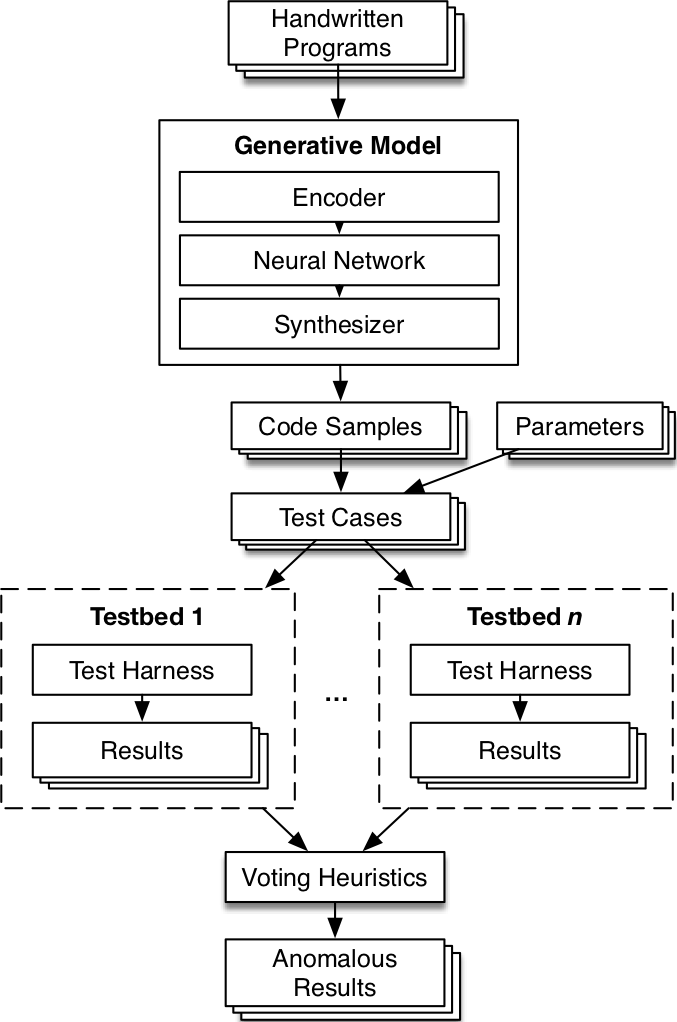
\includegraphics[width=.7\columnwidth]{img/deepsmith}
  \caption[DeepSmith system overview]{%
    DeepSmith system overview. Handwritten programs are used to derive a generative model; from which code samples are produced and parameterised to make test cases. Test cases are broadcast to multiple testbeds, and voting heuristics used to determine the testbeds that deviate from the majority, exposing anomalous results.
  }%
  \label{fig:deepsmith}
\end{figure}


\subsection{Generative Model}

Generating test cases for compilers is hard because their inputs are highly structured. Producing text with the right structure requires expert knowledge and a significant engineering effort, which has to be repeated from scratch for each new language. Instead, the proposed approach frames the problem as an unsupervised machine learning task, extending prior work of Chapter~\ref{chap:clgen} in employing state-of-the-art deep learning techniques to build models for how humans write programs. The approach is inspired by breakthrough results in modelling challenging and high dimensional data sets through unsupervised learning~\cite{Raghu2016,Radford2016b,Bowman2015}. Contrary to existing tools, this approach does not require expert knowledge of the target language and is only a few hundred lines of code.


\paragraph*{Handwritten Programs}

The generative model needs to be trained on a \emph{seed corpus} of example programs. The assembly of this corpus is automated by mining 10k OpenCL kernels from open source repositories on GitHub. An \emph{oracle compiler} (LLVM 3.9) is used to statically check each downloaded source file, discarding files that are not well-formed. The main purpose of this step is to remove the need to manually check that each file selected from GitHub does indeed contain OpenCL. A downside is that any training candidate which triggers a bug in the LLVM 3.9's front end will not be included. However, this did not prevent the system from uncovering errors in that compiler (Section~\ref{subsec:clangs}).

This corpus, exceeding one million lines of code, is used as a representative sample of OpenCL code from which a generative model can be derived.

As in Chapter~\ref{chap:clgen}, semantic-preserving transformations are employed to simplify the training programs. First, each source file is preprocessed to expand macros and remove conditional compilation and comments. Then, all user-declared identifiers are renamed using an arbitrary, but consistent pattern based on their order of declaration: $\{a,\allowbreak b,\allowbreak c,\allowbreak \ldots,\allowbreak aa,\allowbreak ab,\allowbreak ac,\allowbreak \ldots\}$ for variables and $\{A,\allowbreak B,\allowbreak C,\allowbreak \ldots,\allowbreak AA,\allowbreak AB,\allowbreak AC,\allowbreak \ldots\}$ for functions. This ensures a consistent naming convention, without modifying program behaviour. Finally, a uniform code style is enforced to ensure consistent use of braces, parentheses, and white space. These rewriting simplifications give more opportunities for the model to learn the structure and deeper aspects of the language and speed up the learning. On the other hand, some bugs in the preprocessor or front-end might no longer be discoverable. For the purpose of fuzzing OpenCL compilers, this was reasoned as an acceptable trade-off. For languages where the corpus may be many orders of magnitude larger, for example, C or Java, it may be possible to construct effective models without these modifications.


\paragraph*{Encoder}

Source code is encoded as a sequence of integers for interpretation by artificial neural networks, where each integer is an index into a predetermined vocabulary. In~\cite{Jozefowicz2016a}, a character based vocabulary is used. This minimises the size of the vocabulary but leads to long sequences which are harder to extract structure from. In~\cite{Allamanis2013a}, a token based vocabulary is used. This leads to shorter sequences, but causes an explosion in the vocabulary size, as every identifier and literal must be represented uniquely.

A hybrid, partially tokenised vocabulary approach is developed. This allows common multi-character sequences such as \texttt{float} and \texttt{if} to be represented as unique vocabulary items, while literals and other infrequently used words are encoded at the character level.

First, a candidate vocabulary $V_c$ is assembled for the OpenCL programming language containing the 208 data types, keywords, and language builtins of the OpenCL programming language. From this, the subset of the candidate vocabulary $V \in V_c$ which is required to encode a corpus of 45k lines of GPGPU benchmark suite kernels is derived. Beginning with the first character in the corpus, the algorithm consumes the longest matching sequence from the candidate vocabulary. This process continues until every character in the corpus has been consumed, illustrated in Algorithm~\ref{alg:maxmunch-tokenization}. The resulting derived vocabulary consists of 128 symbols which are used to encode new program sources.

\begin{algorithm}
  \begin{algorithmic}[1]
\Require Candidate vocabulary $V_c$, string $S$.
\Ensure Vocabulary $V$.
\State $V \gets \varnothing$\algorithmiccomment{Initialise empty derived vocabulary}
\State $i \gets 1$
\While{$S \ne ``''$}\algorithmiccomment{While input not fully processed}
  \State $i \gets i + 1$\algorithmiccomment{Advance to next character}
  \State $c \gets [S^{(1)}, \ldots, S^{(i)}]$\algorithmiccomment{Read token from input}
    \If{$! IsValidPrefix(c, V_c)$}\algorithmiccomment{If token is not legal}
      \State $c \gets FindLongestSubstring(c, V_c)$\algorithmiccomment{Revert to last legal token}
      \State $S \gets [S^{(|c|)}, \ldots, S^{(|S|)}]$\algorithmiccomment{Pop token from input}
      \State $V \gets V \cup \{ c \}$\algorithmiccomment{Add token to vocabulary}
    \State $i \gets 1$
  \EndIf
\EndWhile
\end{algorithmic}

  \caption[Deriving a vocabulary from a string]{%
    Deriving a hybrid token- and character-level vocabulary from a string.%
  }
  \label{alg:maxmunch-tokenization}
\end{algorithm}


\paragraph*{Neural Network}

The Long Short-Term Memory (LSTM) architecture of Recurrent Neural Network is used to model program code~\cite{Hochreiter1997}. In the LSTM architecture activations are learned with respect not just to their current inputs but to previous inputs in a sequence. In this case, this allows modelling the probability of a token appearing in the text given a history of previously seen tokens. Unlike previous recurrent networks, LSTMs employ a \emph{forget gate} with a linear activation function, allowing them to avoid the \emph{vanishing gradients} problem~\cite{Pacanu2013}. This makes them effective at learning complex relationships over long sequences~\cite{Lipton2015} which is important for modelling program code. Extending the character-based model of Chapter~\ref{chap:clgen}, LSTM networks are employed to model the token-vocabulary distribution over the encoded corpus.

Compared to prior character-based models, the hybrid token vocabulary caused models to respond differently to model parameters. Initial experiments using different model parameters revealed that a two-layer LSTM network of 512 nodes per layer provided a good trade-off between the fidelity of the learned distribution and the size of the network, which limits the rate of training and inference. The network is trained using Stochastic Gradient Descent for 50 epochs, with an initial learning rate of 0.002 and decaying by 5\% every epoch. Training the model on the OpenCL corpus took 12 hours using a single NVIDIA Tesla P40. The model is given no prior knowledge of the structure or syntax of a programming language.


\paragraph*{Program Generation}

The trained network is sampled to generate new programs. The model is seeded with the start of a kernel (identified in OpenCL using the keywords \texttt{kernel void}) and sampled token-by-token. A ``bracket depth'' counter is incremented or decremented upon production of \texttt{\{} or \texttt{\}} tokens respectively so that the end of the kernel is detected and sampling halted. Unlike in Chapter~\ref{chap:clgen}, there is no support for forcing kernel specifications, and there is no upper bound on the length of a sample. The generated sequence of tokens is then decoded back to text and used for compiler testing.


\subsection{Test Harness\label{sec:test-harness}}

OpenCL is an embedded compute kernel language, requiring host code to compile, execute, and transfer data between the host and device. For the purpose of compiler fuzzing, this requires a \emph{test harness} to run the generated OpenCL programs. At first, the test harness of CLSmith was used. The harness assumes a kernel with no input and a \texttt{ulong} buffer as its single argument where the result is written. Only 0.2\% of the GitHub kernels share this structure. A more flexible harness was desired so as to test a more expressive range of programs, capable of supporting multi-argument kernels and generating data to use as inputs.

A new harness was developed, extending CLdrive, which first determines the expected arguments from the function prototype and generates host data for them. At the moment, scalars and arrays of all OpenCL primitive and vector types are supported. For a kernel execution across $n$ threads, buffers of size $n$ are allocated for pointer arguments and populated with values {$[1 \ldots n]$}; scalar inputs are given value $n$ since scalar integer arguments are frequently used in OpenCL for specifying buffer sizes.

The training programs from which the generative model is created are real programs, and as such do not share the argument type restrictions. The model, therefore, may generate correct programs for which the driver cannot create example inputs. In this case, a ``compile-only'' stub is used, which only compiles the kernel, without generating input data or executing the compiled kernel.

Unlike the generative model, this test harness is language-specific and the design stems from domain knowledge. Still, it is a relatively simple procedure, consisting of a few hundred lines of Python.


\paragraph*{Test Harness Output Classes}

Executing a test case on a testbed leads to one of seven possible outcomes, illustrated in Figure~\ref{fig:test-process}. A \emph{build failure} occurs when the online compilation of an OpenCL kernel fails, usually accompanied by an error diagnostic. A \emph{build crash} or \emph{build timeout} outcome occurs if the compiler crashes or fails to produce a binary within 60 seconds, respectively. For compile-only test cases, a \emph{pass} is achieved if the compiler produces a binary. For test cases in which the kernel is executed, kernel execution leads to one of three potential outcomes: \emph{runtime crash} if the program crashes, \emph{timeout} if the kernel fails to terminate within 60 seconds, or \emph{pass} if the kernel terminates gracefully and computes an output.

\begin{figure}
  \centering %
  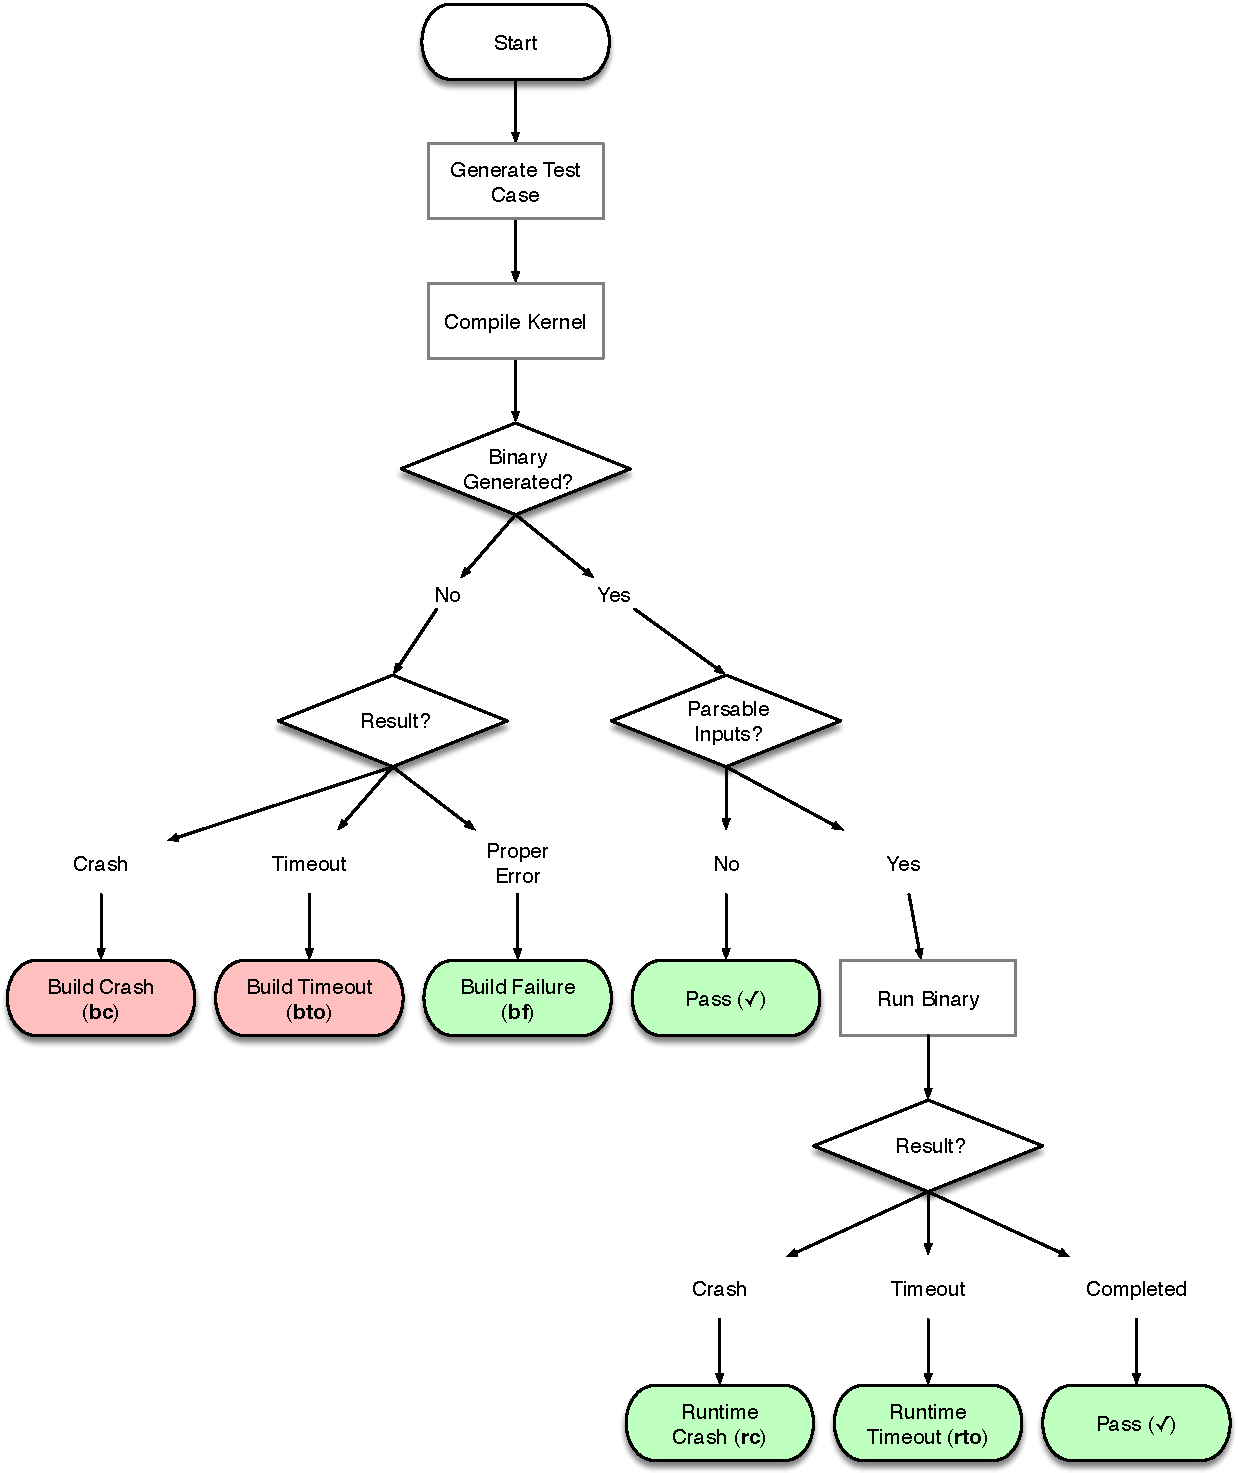
\includegraphics[width=\columnwidth]{img/testcase-flow-chart}
  \caption[Test case execution, and possible results]{%
    Test case execution, and possible results. Generating and executing a test case leads to one of six possible outcomes. Of these, build crashes and build timeouts are considered errors. In the remaining four cases, differential testing may be used to determine if the outcome is anomalous.%
  }%
  \label{fig:test-process}
\end{figure}


\subsection{Voting Heuristics for Differential Testing}

Established Differential Testing methodologies are employed to expose compiler defects. As in prior work, voting on the output of programs across compilers has been used to circumvent the \emph{oracle problem} and detect miscompilations~\cite{McKeeman1998}. However, this approach is extended to describe not only miscompilations, but also anomalous build failures and crashes.

\newpage
When evaluating the outcomes of test cases, build crash (\bc) and build timeout (\bto) outcomes are of immediate interest, indicative of erroneous compiler behaviour (examples may be found in Section~\ref{subsec:compile-time-defects}). For all other outcomes, \emph{differential tests} are required to confirm anomalous behaviour. The idea is to identify test cases where there is a majority outcome -- i.e. for which some fraction of the testbeds behaves the same -- but some testbed deviates. The presence of the majority increases the likelihood that there is a `correct' behaviour for the test case. In this work, a majority fraction of $\ceil{\frac{2}{3}n}$ is used, where $n$ is the number of testbeds.

An \emph{anomalous build failure} (\abf) or \emph{anomalous runtime crash} (\arc) occurs if, for a given test case, the majority of testbeds execute successfully, and a testbed yields a compilation error or runtime crash. An \emph{anomalous wrong-output} (\awo) occurs if, for a given test case, the majority of testbeds execute successfully, producing the same output values, and a testbed yields a result which differs from this majority output. Anomalous wrong-output results are indicative of \emph{miscompilations}, a particularly hard to detect class of bug in which the compiler silently emits wrong code. CSmith is designed specifically to target this class of bug.


\paragraph*{False Positives for Anomalous Runtime Behaviour}

Generated programs may contain undefined or non-deterministic behaviour which will incorrectly be labelled as anomalous. CSmith circumvents this problem by performing complex analyses during generation so as to minimise the chance of producing programs with undefined behaviour. Although similar analyses could be created as filters for DeepSmith, a simpler approach is taken, filtering only the few types of non-deterministic behaviour that have been actually observed to happen in practice.

Data races, out-of-bounds and uninitialised accesses are filtered using GPUverify~\cite{Betts2012} and Oclgrind~\cite{Price2015}. Some compiler warnings provide a strong indication of non-deterministic behaviour (e.g. comparison between pointer and integer) -- these warnings are checked for and filtered accordingly.

Floating point operations in OpenCL are imprecise, so kernels can produce different output on different testbeds. For this reason, CSmith and CLSmith do not support floating point operations. DeepSmith permits floating point operations but since it cannot apply differential testing on the outputs, it can detect all results except for the \emph{anomalous wrong-output} results.

The last type of undefined behaviour observed comes from division by zero and related mathematical functions which require non-zero values. A simple detection and filtering heuristic was applied -- the input values are changed and the output is checked to see if it remains anomalous. While theoretically insufficient, in practice no false positives have been found to remain.


\section{Experimental Setup}
\label{sec:deepsmith-experimental-setup}

This section describes the experimental parameters used for a testing campaign of OpenCL compilers.


\subsection{OpenCL Systems}

Testing was conducted on 10 OpenCL systems, summarised in Table~\ref{tab:deepsmith-platforms}. A broad range of hardware was covered: 3 GPUs, 4 CPUs, a co-processor, and an emulator. 7 of the compilers tested are commercial products, 3 of them are open source. This suite of systems includes both combinations of different drivers for the same device, and different devices using the same driver.

\begin{table}
  \centering %
  \subfloat[][]{\rowcolors{2}{gray!25}{white}
\begin{tabular}{ | c l l l l | }
	\hline
	\rowcolor{gray!50}
	\textbf{\#. } & \textbf{Platform} & \textbf{Device} & \textbf{Driver} & \textbf{OpenCL} \\
	\hline
	1 & NVIDIA CUDA & GeForce GTX 1080 & 375.39 & 1.2 \\
	2 & NVIDIA CUDA & GeForce GTX 780 & 361.42 & 1.2 \\
	3 & Beignet & Intel HD Haswell GT2 & 1.3 & 1.2 \\
	4 & Intel OpenCL & Intel E5-2620 v4 & 1.2.0.25 & 2.0 \\
	5 & Intel OpenCL & Intel E5-2650 v2 & 1.2.0.44 & 1.2 \\
	6 & Intel OpenCL & Intel i5-4570 & 1.2.0.25 & 1.2 \\
	7 & Intel OpenCL & Intel Xeon Phi & 1.2 & 1.2 \\
	8 & POCL & POCL (Intel E5-2620) & 0.14 & 1.2 \\
	9 & Codeplay & ComputeAorta (Intel E5-2620) & 1.14 & 1.2 \\
	10 & Oclgrind & Oclgrind Simulator & 16.10 & 1.2 \\
	\hline
\end{tabular}
}\\%
  \subfloat[][]{\rowcolors{2}{gray!25}{white}
\begin{tabular}{ | c l l R{2.2cm} | R{2.75cm} | }
  \hline
  \rowcolor{gray!50}
  \textbf{\#. } & \textbf{Operating system} & \textbf{Device Type} & \textbf{Open Source?} & \textbf{Bug Reports Submitted} \\
  \hline
  1 & Ubuntu 16.04 64bit & GPU & & 8 \\
  2 & openSUSE 13.1 64bit & GPU & & 1 \\
  3 & Ubuntu 16.04 64bit & GPU & Yes & 13 \\
  4 & Ubuntu 16.04 64bit & CPU & & 6 \\
  5 & CentOS 7.1 64bit & CPU & & 1 \\
  6 & Ubuntu 16.04 64bit & CPU & & 5 \\
  7 & CentOS 7.1 64bit & Accelerator & & 3 \\
  8 & Ubuntu 16.04 64bit & CPU & Yes & 22 \\
  9 & Ubuntu 16.04 64bit & CPU & & 1 \\
  10 & Ubuntu 16.04 64bit & Emulator & Yes & 7 \\
  \hline
\end{tabular}
} %
  \caption[OpenCL systems and the number of bug reports submitted to date]{%
    OpenCL systems and the number of bug reports submitted to date (22\% of which have been fixed, the remainder are pending). For each system, two testbeds are created, one with compiler optimisations, the other without.%
  }
  \label{tab:deepsmith-platforms}
\end{table}


\subsection{Testbeds}

For each OpenCL system, two testbeds are created. In the first, the compiler is run with optimisations disabled. In the second, optimisations are enabled. Each testbed is then a triple, consisting of \emph{\textless device, driver, is\_optimised\textgreater} settings. This mechanism gives 20 testbeds to evaluate.


\subsection{Test Cases}

Inputs are created for each generated program as described in Section~\ref{sec:test-harness}. The test harness is parameterised by a number of threads to use. Two test cases are generated, one using one thread, the other using 2048 threads. A test case is then a triple, consisting of \emph{\textless program, inputs, threads\textgreater} settings.

\subsection{Bug Search Time Allowance}

DeepSmith and CLSmith are compared by allowing both to run for 48 hours on each of the 20 testbeds. CLSmith used its default configuration. The total runtime for a test case consists of the generation and execution time.


\section{Evaluation}
\label{sec:deepsmith-eval}

This section reports on the results of DeepSmith testing of the 10 OpenCL systems from Table~\ref{tab:deepsmith-platforms}, in which each ran for 48 hours. Bugs were found in all the compilers tested --- every compiler crashed, and every compiler generated programs which either crash or silently compute the wrong result. To date, 67 unique bug reports have been submitted to compiler vendors. This section first contains a qualitative analysis of compile-time and runtime defects found, followed by a quantitative comparison of the approach against the state-of-the-art in OpenCL compiler fuzzing --- CLSmith~\cite{Lidbury2015a}. DeepSmith is able to identify a broad range of defects, many of which CLSmith cannot, for only a fraction of the engineering effort. Finally, this section contains a quantitative analysis of compiler robustness over time, using the compiler crash rate of every LLVM release in the past two years as a metric of compiler robustness. The findings show that progress is good, compilers are becoming more robust, yet the introduction of new features and regressions ensures that compiler validation remains a moving target.

Unless stated otherwise, DeepSmith code listings are presented verbatim, with only minor formatting changes applied to preserve space. No test case reduction, either manual or automatic, was needed.

For the remainder of this chapter, testbeds are identified using the OpenCL system number from Table~\ref{tab:deepsmith-platforms}, suffixed with $+$, $-$, or $\pm$ to denote optimisations on, off, or either, respectively.


\subsection{Compile-time Defects}%
\label{subsec:compile-time-defects}

OpenCL is typically compiled online, which amplifies the significance of detecting compile-time defects, as they may not be discovered until code has been shipped to customers. Numerous cases were found where DeepSmith kernels trigger a crash in the compiler (and as a result, the host process), or cause the compiler to loop indefinitely. In the testing time allotted, DeepSmith uncovered 199 unique unreachable code failures, 31 different compiler assertions, and 114 distinct stack traces caused by other compiler crashes.

\newsavebox{\ParserFailOne}
\begin{lrbox}{\ParserFailOne}
  \begin{minipage}{\textwidth}
    \begin{minted}{opencl_lexer.py:OpenCLLexer -x}
void A(){(global a*)()
    \end{minted}
  \end{minipage}
\end{lrbox}

\newsavebox{\ParserFailTwo}
\begin{lrbox}{\ParserFailTwo}
  \begin{minipage}{\textwidth}
    \begin{minted}{opencl_lexer.py:OpenCLLexer -x}
void A(){void* a; uint4 b=0; b=(b>b)?a:a
    \end{minted}
  \end{minipage}
\end{lrbox}

\newsavebox{\ParserFailThree}
\begin{lrbox}{\ParserFailThree}
  \begin{minipage}{\textwidth}
    \begin{minted}{opencl_lexer.py:OpenCLLexer -x}
void A(){double2 k; return (float4)(k,k,k,k)
    \end{minted}
  \end{minipage}
\end{lrbox}

\begin{figure}
  \centering %
  \subfloat[Reduced from 48 line kernel.]{%
  \noindent\mbox{\parbox{\columnwidth}{\usebox{\ParserFailOne}}}%
  }\\%
  \subfloat[Reduced from 52 line kernel.]{%
  \noindent\mbox{\parbox{\columnwidth}{\usebox{\ParserFailTwo}}}%
  }\\%
  \subfloat[Reduced from 68 line kernel.]{%
  \noindent\mbox{\parbox{\columnwidth}{\usebox{\ParserFailThree}}}%
  }\\%
  \caption[Example codes which crash parsers]{%
    Example codes which crash OpenCL compilers during parsing.%
  }
  \label{lst:parser-crashes}
\end{figure}


\subsubsection{Semantic Analysis Failures}

Compilers should produce meaningful diagnostics when inputs are invalid, yet dozens of compiler defects were discovered attributable to improper or missing error handling. Many generation and mutation based approaches to compiler validation have focused solely on testing under \emph{valid inputs}. As such, this class of bugs may go undiscovered. Compared to these approaches, DeepSmith may contribute a significant improvement for generating plausibly-erroneous code over prior random-enumeration approaches.

The use of undeclared identifiers is a core error diagnostic which one would expect to be robust in a mature compiler. DeepSmith discovered cases in which the presence of undeclared identifiers causes the Testbeds $10\pm$ compiler to crash. For example, the undeclared identifier \texttt{c} in Figure~\ref{lst:oclgrind-uncorrected-typos} raises an assertion during semantic analysis of the AST when used as an array index.

\newsavebox{\OclgrindUncorrectedTypos}
\begin{lrbox}{\OclgrindUncorrectedTypos}
  \begin{minipage}{\textwidth}
    \begin{minted}{opencl_lexer.py:OpenCLLexer -x}
kernel void A(global float* a, global float* b) {
  a[0] = max(a[c], b[2]);
}
    \end{minted}
  \end{minipage}
\end{lrbox}

\newsavebox{\NvidiaRecursionSegfault}
\begin{lrbox}{\NvidiaRecursionSegfault}
  \begin{minipage}{\textwidth}
    \begin{minted}{opencl_lexer.py:OpenCLLexer -x}
kernel void A(float4 a, global float4* b,
              global float4* c, unsigned int d,
              global double* e, global int2* f,
              global int4* g, constant int* h,
              constant int* i) {
  A(a, b, c, d, d, e, f, g, h);
}
    \end{minted}
  \end{minipage}
\end{lrbox}

\newsavebox{\IntelGtDoubleAssertion}
\begin{lrbox}{\IntelGtDoubleAssertion}
  \begin{minipage}{\textwidth}
    \begin{minted}{opencl_lexer.py:OpenCLLexer -x}
kernel void A(read_only image2d_t a,
              global double2* b) {
  b[0] = get_global_id(0);
}
    \end{minted}
  \end{minipage}
\end{lrbox}

\newsavebox{\BeignetScalarizeInsert}
\begin{lrbox}{\BeignetScalarizeInsert}
  \begin{minipage}{\textwidth}
    \begin{minted}{opencl_lexer.py:OpenCLLexer -x}
kernel void A(global float4* a) {
  a[get_local_id(0) / 8][get_local_id(0)] =
      get_local_id(0);
}
    \end{minted}
  \end{minipage}
\end{lrbox}

\newsavebox{\AlmostEverythingCrash}
\begin{lrbox}{\AlmostEverythingCrash}
  \begin{minipage}{\textwidth}
    \begin{minted}{opencl_lexer.py:OpenCLLexer -x}
kernel void A() {
  __builtin_astype(d, uint4);
}
    \end{minted}
  \end{minipage}
\end{lrbox}

\begin{figure}
  \centering %
  \subfloat[Testbeds $10\pm$ assertion \emph{Uncorrected typos!} during semantic analysis.]{%
    \noindent\mbox{\parbox{\columnwidth}{\usebox{\OclgrindUncorrectedTypos}}}%
    \label{lst:oclgrind-uncorrected-typos}
  }\\%
  \subfloat[Testbeds $1\pm$, $2\pm$ segmentation fault due to implicit address space conversion.]{%
    \noindent\mbox{\parbox{\columnwidth}{\usebox{\NvidiaRecursionSegfault}}}%
    \label{lst:nvidia-recursion-segfault}
  }\\%
  \subfloat[Testbeds $3\pm$ assertion \emph{sel.hasDoubleType()} during code generation.]{%
    \noindent\mbox{\parbox{\columnwidth}{\usebox{\IntelGtDoubleAssertion}}}%
    \label{lst:intel-gt2-double-assertion}
  }\\%
  \subfloat[Testbeds $3\pm$ assertion \emph{scalarizeInsert} during code generation.]{%
    \noindent\mbox{\parbox{\columnwidth}{\usebox{\BeignetScalarizeInsert}}}%
    \label{lst:beignet-scalarize-insert}
  }\\%
  \subfloat[Of the 10 compilers tested, 6 crash with segfault when compiling this kernel.]{%
    \noindent\mbox{\parbox{\columnwidth}{\usebox{\AlmostEverythingCrash}}}%
    \label{lst:almost-everything-crash}
  }\\%
  \caption[Example OpenCL kernels which crash compilers]{%
    Example OpenCL kernels which crash compilers.%
  }%
\end{figure}

Type errors were an occasional cause of compile-time defects. Figure~\ref{lst:nvidia-recursion-segfault} induces a crash in NVIDIA compilers due to an implicit conversion between global to constant address qualifiers. Worse, Testbeds $3\pm$ were found to loop indefinitely on some kernels containing implicit conversions from a pointer to an integer, as shown in Figure~\ref{lst:beignet-ptr-int-spin}. While spinning, the compiler would utilise 100\% of the CPU and consume an increasing amount of host memory until the entire system memory is depleted and the process crashes.

Occasionally, incorrect program semantics will remain undetected until late in the compilation process. Both Figures~\ref{lst:intel-gt2-double-assertion} and~\ref{lst:beignet-scalarize-insert} pass the type checker and semantic analysis, but trigger compiler assertions during code generation.

An interesting yet unintended by-product of having trained DeepSmith on thousands of real-world examples is that the model learned to occasionally generate compiler-specific code, such as invoking compiler intrinsics. The quality of error handling on these builtins was found to vary wildly. For example, Figure~\ref{lst:almost-everything-crash} silently crashes 6 of the 10 compilers, which, to the best of my knowledge, makes DeepSmith the first random program generator to induce a defect through exploiting compiler-specific functionality.


\subsubsection{Parser Failures}

Parser development is a mature and well-understood practice. Still, parser errors were discovered in several compilers. Each of the code samples in Figure~\ref{lst:parser-crashes} induce crash errors during parsing of compound statements in both Testbeds $5\pm$ and $7\pm$. For space, the listings have been hand-reduced to minimal code samples, which have been reported to Intel. Each reduction took around 6 edit-compile steps, taking less than 10 minutes. In total, 100 distinct programs have been generated which crash compilers during parsing.

\newsavebox{\BeignetPtrIntSpin}
\begin{lrbox}{\BeignetPtrIntSpin}
  \begin{minipage}{\textwidth}
    \begin{minted}{opencl_lexer.py:OpenCLLexer -x}
kernel void A(global int* a) {
  int b = get_global_id(0);
  a[b] = (6 * 32) + 4 * (32 / 32) + a;
}
    \end{minted}
  \end{minipage}
\end{lrbox}

\newsavebox{\NvidiaOptLoopHang}
\begin{lrbox}{\NvidiaOptLoopHang}
  \begin{minipage}{\textwidth}
    \begin{minted}{opencl_lexer.py:OpenCLLexer -x}
kernel void A(global float* a, global float* b,
              global float* c) {
  int d, e, f;
  d = get_local_id(0);
  for (int g = 0; g < 100000; g++)
    barrier(1);
}
    \end{minted}
  \end{minipage}
\end{lrbox}

\newsavebox{\XeonPhiSpin}
\begin{lrbox}{\XeonPhiSpin}
  \begin{minipage}{\textwidth}
    \begin{minted}{opencl_lexer.py:OpenCLLexer -x}
kernel void A(global unsigned char* a,
              unsigned b) {
  a[get_global_id(0)] %= 42;
  barrier(1);
}
    \end{minted}
  \end{minipage}
\end{lrbox}

\newsavebox{\IntelOptLoopHang}
\begin{lrbox}{\IntelOptLoopHang}
  \begin{minipage}{\textwidth}
    \begin{minted}{opencl_lexer.py:OpenCLLexer -x}
    kernel void A(global int* a) {
      int b = get_global_id(0);
      while (b < 512) { }
    }
    \end{minted}
  \end{minipage}
\end{lrbox}

\begin{figure}
  \centering %
  \subfloat[Testbeds $3\pm$ loop indefinitely, leaking memory until the entire system memory is depleted and the process crashes.]{%
  \noindent\mbox{\parbox{\columnwidth}{\usebox{\BeignetPtrIntSpin}}}%
  \label{lst:beignet-ptr-int-spin}
  }\\%
  \subfloat[Testbed $1+$ hangs during optimisation of kernels with large loop bounds. Testbeds $1-$ and $2\pm$ compile in under 1 second.]{%
  \noindent\mbox{\parbox{\columnwidth}{\usebox{\NvidiaOptLoopHang}}}%
  \label{lst:nvidia-opt-loop-hang}
  }\\%
  \subfloat[Testbeds $7\pm$ loops indefinitely, consuming 100\% CPU usage.]{%
  \noindent\mbox{\parbox{\columnwidth}{\usebox{\XeonPhiSpin}}}%
  \label{lst:xeon-phi-spin}
  }\\%
  \subfloat[Testbeds $4+$, $5+$, $6+$, $7+$ hang during optimisation of kernels with non-terminating loops.]{%
  \noindent\mbox{\parbox{\columnwidth}{\usebox{\IntelOptLoopHang}}}%
  \label{lst:intel-inf-loop}
  }\\%
  \caption[Example kernels which hang compilers]{%
    Example OpenCL kernels which hang compilers.%
  }%
  \label{lst:compiler-hangs}
\end{figure}


\subsubsection{Compiler Hangs}

As expected, some compile-time defects are optimisation sensitive. Testbed $1+$ hangs on large loop bounds, shown in Figure~\ref{lst:nvidia-opt-loop-hang}. All commercial Intel compilers  tested hang during optimisation of non-terminating loops (Figure~\ref{lst:intel-inf-loop}).

Testbeds $7\pm$ loop indefinitely during compilation of the simple OpenCL kernel in Figure~\ref{lst:xeon-phi-spin}.


\subsubsection{Other errors}

Some compilers are more permissive than others. Testbeds~$4\pm$, $6\pm$, $9\pm$ reject out-of-range literal values e.g. \texttt{int i = 0xFFFFFFFFFFFFFFFFFFFFFFFF}, whilst Testbeds $3\pm$, $5\pm$, $7\pm$, $8\pm$, and $10\pm$ interpret the literal as an \texttt{unsigned long long} and implicitly cast to an integer value of \texttt{-1}. Testbeds $1\pm$, $2\pm$ emit no warning.

Testbeds~$1\pm$, $2\pm$, $3\pm$ rejected address space qualifiers on automatic variables, where all other testbeds successfully compiled and executed.

On Testbeds~$3\pm$, the statement \texttt{int n = mad24(a, (32), get\_global\_size(0));} (a call to a maths builtin with mixed types) is rejected as ambiguous.


\newsavebox{\IntelSizetIntUnreduced}
\begin{lrbox}{\IntelSizetIntUnreduced}
  \begin{minipage}{\textwidth}
    \begin{minted}{opencl_lexer.py:OpenCLLexer -x}
kernel void A(global double* a, global double* b,
              global double* c, int d, int e) {
  double f;
  int g = get_global_id(0);
  if (g < e - d - 1)
    c[g] = (((e) / d) % 5) % (e + d);
}
    \end{minted}
  \end{minipage}
\end{lrbox}

\newsavebox{\OclgrindRaceSwitch}
\begin{lrbox}{\OclgrindRaceSwitch}
  \begin{minipage}{\textwidth}
    \begin{minted}{opencl_lexer.py:OpenCLLexer -x}
kernel void A(global int* a, global int* b) {
  switch (get_global_id(0)) {
  case 0:
    a[get_global_id(0)]=b[get_global_id(0)+13];
    break;
  case 2:
    a[get_global_id(0)]=b[get_global_id(0)+11];
    break;
  case 6:
    a[get_global_id(0)]=b[get_global_id(0)+128];
  }
  barrier(2);
}
    \end{minted}
  \end{minipage}
\end{lrbox}

\newsavebox{\BeignetTernary}
\begin{lrbox}{\BeignetTernary}
  \begin{minipage}{\textwidth}
    \begin{minted}{opencl_lexer.py:OpenCLLexer -x}
kernel void A(global int* a, global int* b,
              global int* c) {
  c[0] = (a[0] > b[0]) ? a[0] : 0;
  c[2] = (a[3] <= b[3]) ? a[4] : b[5];
  c[4] = (a[4] <= b[5]) ? a[7] : b[7];
  c[7] = (a[7] < b[0]) ? a[0] : (a[0] > b[1]);
}
    \end{minted}
  \end{minipage}
\end{lrbox}

\begin{figure}
  \centering %
  \subfloat[Testbeds $4+$, $6+$ incorrectly optimise the \texttt{if} statement, causing the conditional branch to execute (it shouldn't). This pattern of integer comparison to thread ID is widely used.]{%
    \noindent\mbox{\parbox{\columnwidth}{\usebox{\IntelSizetIntUnreduced}}}%
    \label{lst:intel-size_t-int-unreduced}
  }\\%
  \subfloat[A race condition in \texttt{switch} statement evaluation causes $10\pm$ to sporadically crash when executed with a number of threads $> 1$.]{%
    \noindent\mbox{\parbox{\columnwidth}{\usebox{\OclgrindRaceSwitch}}}%
    \label{lst:oclgrind-race-switch}
  }\\%
  \caption[Example kernels which are miscompiled]{%
    Example OpenCL kernels which are miscompiled.%
  }%
\end{figure}

\newsavebox{\PoclUndefinedSymbols}
\begin{lrbox}{\PoclUndefinedSymbols}
  \begin{minipage}{\textwidth}
    \begin{minted}{opencl_lexer.py:OpenCLLexer -x}
kernel void A(local int* a) {
  for (int b = 0; b < 100; b++)
    B(a);
}
    \end{minted}
  \end{minipage}
\end{lrbox}

\begin{figure}
  \centering %
  \subfloat[Testbeds $3\pm$ silently miscompile ternary assignments in which the operands are different global buffers.]{%
    \noindent\mbox{\parbox{\columnwidth}{\usebox{\BeignetTernary}}}%
    \label{lst:beig-ternary-ops}
  }\\%
  \subfloat[Compilation should fail due to call to undefined function \texttt{B()}; Testbeds $8\pm$ silently succeed then crash upon kernel execution.]{%
    \noindent\mbox{\parbox{\columnwidth}{\usebox{\PoclUndefinedSymbols}}}%
    \label{lst:pocl-undefined-symbols}
  }\\%
  \caption[Further example kernels which are miscompiled]{%
    Further example OpenCL kernels which are miscompiled.%
  }%
\end{figure}


\subsection{Runtime Defects}

Prior work on compiler test case generation has focused on extensive stress-testing of compiler middle-ends to uncover miscompilations~\cite{Chen2014a}. CSmith, and by extension, CLSmith, specifically targets this class of bugs. Grammar-based enumeration is highly effective at this task, yet is bounded by the expressiveness of the grammar. Here, examples are provided of bugs which cannot currently be discovered by CLSmith.


\subsubsection{Thread-dependent Flow Control}

A common pattern in OpenCL is to obtain the thread identity, often as an \texttt{int}, and to compare this against some fixed value to determine whether or not to complete a unit of work (46\% of OpenCL kernels on GitHub use this ($tid \rightarrow$ int, \texttt{if (tid < \ldots) \{\ldots\}}) pattern). DeepSmith, having modelled the frequency with which this pattern occurs in real handwritten code, generates many permutations of this pattern. And in doing so, exposed a bug in the optimiser of Testbeds $4+$ and $6+$ which causes the \texttt{if} branch in Figure~\ref{lst:intel-size_t-int-unreduced} to be erroneously executed when the kernel is compiled with optimisations enabled. This issue has been reported to Intel. CLSmith does not permit the thread identity to modify control flow, rendering such productions impossible.

Figure~\ref{lst:oclgrind-race-switch} shows a simple program in which thread identity determines the program output. This test case was found to sporadically crash Testbeds~$10\pm$, an OpenCL device simulator and debugger. Upon reporting to the developers, the underlying cause was quickly diagnosed as a race condition in \texttt{switch} statement evaluation and fixed within a week.


\subsubsection{Kernel Inputs}

CLSmith kernels accept a single buffer parameter into which each thread computes its result. This fixed prototype limits the ability to detect bugs which depend on input arguments. Figure~\ref{lst:beig-ternary-ops} exposes a bug of this type. Testbeds $3\pm$ will silently miscompile ternary operators when the ternary operands consist of values stored in multiple different global buffers. CLSmith, with its fixed single input prototype, is unable to discover this bug.


\subsubsection{Latent Compile-time Defects}

Sometimes, invalid compiler inputs may go undetected, leading to runtime defects only upon program execution. Since CLSmith enumerates only well-formed programs, this class of bugs cannot be discovered.

Figure~\ref{lst:pocl-undefined-symbols} exposes a bug in which a kernel containing an undefined symbol will successfully compile without warning on Testbeds~$8\pm$, then crash the program when attempting to run the kernel. This issue has been reported to the developers and fixed.


\subsection{Comparison to State-of-the-art}

This section provides a quantitative comparison of the bug-finding capabilities of DeepSmith and CLSmith.


\subsubsection{Results Overview}

Tables~\ref{tab:megatable-clsmith} and~\ref{tab:megatable-deepsmith} shows the results of 48 hours of consecutive testing for all Testbeds using CLSmith and DeepSmith, respectively. An average of 15k CLSmith and 91k DeepSmith test cases were evaluated on each Testbed, taking 12.1s and 1.90s per test case respectively. There are three significant factors providing the sixfold increase in testing throughput achieved by DeepSmith over CLSmith: test cases are faster to generate, test cases are less likely to timeout (execute for 60 seconds without termination), and the test cases which do not timeout execute faster.

Figure~\ref{fig:deepsmith-vs-clsmith}a shows the generation and execution times of DeepSmith and CLSmith test cases, excluding timeouts\footnote{If timeouts are included then the performance improvement of DeepSmith is $6.5\times$ with the execution times being $11\times$ faster. However, this number grows as the arbitrary timeout threshold is changed, so for fairness timeouts have been excluded.}. DeepSmith generation time grows linearly with program length and is on average $2.45\times$ faster than CLSmith. Test case execution is on average $4.46\times$ faster than CLSmith.

\begin{figure}
  \centering %
  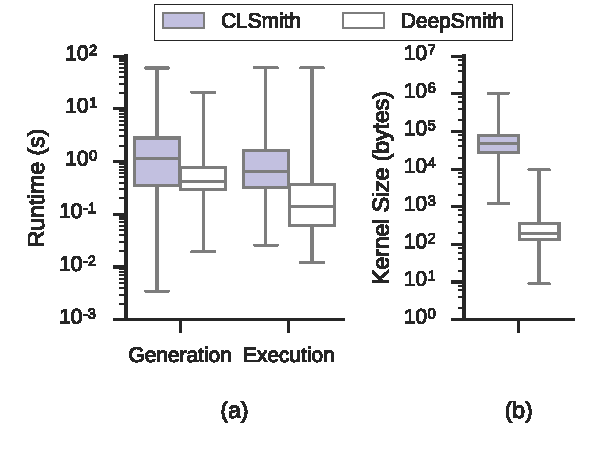
\includegraphics[width=.72\columnwidth]{img/deepsmith-vs-clsmith}%
  \caption[Comparison of DeepSmith and CLSmith runtimes]{%
    Comparison of runtimes (a) and test case sizes (b). DeepSmith test cases are on average evaluated $3.03\times$ faster than CLSmith ($2.45\times$, and $4.46\times$ for generation and execution, respectively), and are two orders of magnitude smaller. Timings do not include the cost of timeouts which would increase the performance gains of DeepSmith by nearly a factor of two.%
  }%
  \label{fig:deepsmith-vs-clsmith}
\end{figure}

The optimisation level generally does not affect testing throughput significantly, with the exception of Testbed~$7+$. Optimisation of large structs is expensive on Testbed~$7+$, and CLSmith test cases use global structs extensively. This is a known issue --- in~\cite{Lidbury2015a} the authors omit large-scale testing on this device for this reason. The use of structs in handwritten OpenCL is comparatively rare --- only 7.1\% of kernels on GitHub use them.

\begin{table}
  \centering %
  \begin{tabular}{| lll | rrrrrrr |}
  \hline
  \rowcolor{gray!50}
  \textbf{\#.} & \textbf{Device} & $\pm$ &
  \bc & \bto & \abf & \arc & \awo & \textbf{\cmark} & \textbf{total} \\
  \hline
  & & $-$ & 0 & 0 & 0 & 2 & 2 & 15628 & 15632  \\
  \multirow{ -2}{*}{1} & \multirow{-2}{*}{GeForce GTX 1080} & $+$ & 0 & 71 & 0 & 6 & 9 & 14007 & 14093 \\
  \rowcolor{gray!25}
  & & $-$ & 0 & 0 & 0 & 28 & 5 & 18220 & 18253 \\
  \rowcolor{gray!25}
  \multirow{-2}{*}{2} & \multirow{-2}{*}{GeForce GTX 780} & $+$ & 26 & 14 & 0 & 0 & 3 & 17654 & 17697 \\
  & & $-$ & 2714 & 2480 & 0 & 0 & 3 & 1121 & 6318 \\
  \multirow{-2}{*}{3} & \multirow{-2}{*}{Intel HD Haswell GT2} & $+$ & 2646 & 2475 & 0 & 0 & 3 & 1075 & 6199 \\
  \rowcolor{gray!25}
  & & $-$ & 0 & 27 & 1183 & 0 & 0 & 16313 & 17523 \\
  \rowcolor{gray!25}
  \multirow{-2}{*}{4} & \multirow{-2}{*}{Intel E5-2620 v4} & $+$ & 487 & 87 & 1130 & 0 & 0 & 17350 & 19054 \\
  & & $-$ & 0 & 11 & 0 & 0 & 0 & 17887 & 17898 \\
  \multirow{-2}{*}{5} & \multirow{-2}{*}{Intel E5-2650 v2} & $+$ & 112 & 175 & 0 & 0 & 0 & 14626 & 14913 \\
  \rowcolor{gray!25}
  & & $-$ & 0 & 14 & 1226 & 0 & 0 & 17118 & 18358 \\
  \rowcolor{gray!25}
  \multirow{-2}{*}{6} & \multirow{-2}{*}{Intel i5-4570} & $+$ & 526 & 63 & 1180 & 0 & 0 & 19185 & 20954 \\
  & & $-$ & 4 & 84 & 0 & 0 & 8 & 13265 & 13361 \\
  \multirow{-2}{*}{7} & \multirow{-2}{*}{Intel Xeon Phi} & $+$ & 42 & 1474 & 0 & 0 & 2 & 3258 & 4776 \\
  \rowcolor{gray!25}
  & & $-$ & 0 & 0 & 0 & 675 & 0 & 17250 & 17925 \\
  \rowcolor{gray!25}
  \multirow{-2}{*}{8} & \multirow{-2}{*}{POCL (Intel E5-2620)} & $+$ & 0 & 3 & 0 & 99 & 5 & 13980 & 14087 \\
  & & $-$ & 0 & 0 & 0 & 0 & 0 & 18479 & 18479 \\
  \multirow{-2}{*}{9} & \multirow{-2}{*}{ComputeAorta} & $+$ & 0 & 0 & 0 & 300 & 11 & 18625 & 18936 \\
  \rowcolor{gray!25}
  & & $-$ & 0 & 0 & 0 & 0 & 0 & 5287 & 5287 \\
  \rowcolor{gray!25}
  \multirow{-2}{*}{10} & \multirow{-2}{*}{Oclgrind Simulator} & $+$ & 0 & 0 & 0 & 0 & 0 & 5334 & 5334 \\
  \hline
\end{tabular}

  \caption[Results from 48 hours of testing using CLSmith]{%
    Results from 48 hours of testing using CLSmith. System \#. as per Table~\ref{tab:deepsmith-platforms}. $\pm$ denotes optimisations off ($-$) vs on ($+$). The remaining columns denote the number of build crash (\bc), build timeout (\bto), anomalous build failure (\abf), anomalous runtime crash (\arc), anomalous wrong-output (\awo), and pass (\textbf{\cmark}) results.
  }
  \label{tab:megatable-clsmith}
\end{table}

\begin{table}
  \centering %
  \setlength\extrarowheight{2pt}
\begin{tabular}{| lll | rrrrrrr |}
  \hline
  \rowcolor{gray!50}
  \textbf{\#.} & \textbf{Device} & $\pm$ &
  \bc & \bto & \abf & \arc & \awo & \textbf{\cmark} & \textbf{total} \\
  \hline
  & & $-$ & 27 & 0 & 3 & 0 & 5 & 62105 & 62140 \\
  \multirow{ -2}{*}{1} & \multirow{-2}{*}{GeForce GTX 1080} & $+$ & 20 & 1 & 1 & 0 & 7 & 57361 & 57390 \\
  \rowcolor{gray!25}
  & & $-$ & 27 & 0 & 3 & 0 & 9 & 87129 & 87168 \\
  \rowcolor{gray!25}
  \multirow{-2}{*}{2} & \multirow{-2}{*}{GeForce GTX 780} & $+$ & 32 & 1 & 1 & 0 & 9 & 82666 & 82709 \\
  & & $-$ & 574 & 200 & 2 & 0 & 12 & 136977 & 137765 \\
  \multirow{-2}{*}{3} & \multirow{-2}{*}{Intel HD Haswell GT2} & $+$ & 569 & 200 & 5 & 0 & 10 & 135430 & 136214 \\
  \rowcolor{gray!25}
  & & $-$ & 57 & 0 & 9 & 1 & 0 & 107982 & 108049 \\
  \rowcolor{gray!25}
  \multirow{-2}{*}{4} & \multirow{-2}{*}{Intel E5-2620 v4} & $+$ & 320 & 147 & 7 & 3 & 0 & 113616 & 114093 \\
  & & $-$ & 152 & 2 & 0 & 0 & 0 & 90882 & 91036 \\
  \multirow{-2}{*}{5} & \multirow{-2}{*}{Intel E5-2650 v2} & $+$ & 170 & 117 & 0 & 0 & 1 & 90478 & 90766 \\
  \rowcolor{gray!25}
  & & $-$ & 73 & 0 & 9 & 2 & 1 & 111240 & 111325 \\
  \rowcolor{gray!25}
  \multirow{-2}{*}{6} & \multirow{-2}{*}{Intel i5-4570} & $+$ & 318 & 140 & 7 & 2 & 1 & 117049 & 117517 \\
  & & $-$ & 68 & 4 & 0 & 0 & 1 & 37171 & 37244 \\
  \multirow{-2}{*}{7} & \multirow{-2}{*}{Intel Xeon Phi} & $+$ & 77 & 47 & 0 & 0 & 0 & 37501 & 37625 \\
  \rowcolor{gray!25}
  & & $-$ & 54 & 1 & 2 & 89 & 3 & 85318 & 85467 \\
  \rowcolor{gray!25}
  \multirow{-2}{*}{8} & \multirow{-2}{*}{POCL (Intel E5-2620)} & $+$ & 46 & 0 & 1 & 104 & 4 & 81267 & 81422 \\
  & & $-$ & 51 & 0 & 1 & 3 & 1 & 112324 & 112380 \\
  \multirow{-2}{*}{9} & \multirow{-2}{*}{ComputeAorta} & $+$ & 59 & 0 & 0 & 48 & 4 & 115323 & 115434 \\
  \rowcolor{gray!25}
  & & $-$ & 2081 & 0 & 0 & 0 & 1 & 73261 & 75343 \\
  \rowcolor{gray!25}
  \multirow{-2}{*}{10} & \multirow{-2}{*}{Oclgrind Simulator} & $+$ & 2265 & 0 & 0 & 0 & 0 & 77959 & 80224 \\
  \hline
\end{tabular}

  \caption[Results from 48 hours of testing using DeepSmith]{%
    Results from 48 hours of testing using DeepSmith. System \#. as per Table~\ref{tab:deepsmith-platforms}. $\pm$ denotes optimisations off ($-$) vs on ($+$). The remaining columns denote the number of build crash (\bc), build timeout (\bto), anomalous build failure (\abf), anomalous runtime crash (\arc), anomalous wrong-output (\awo), and pass (\textbf{\cmark}) results.
  }
  \label{tab:megatable-deepsmith}
\end{table}


\subsubsection{Comparison of Test Cases}

The average CLSmith program is 1189 lines long (excluding headers). CLSmith test cases require reduction in order to expose the underlying bug. An automated approach to OpenCL test case reduction is presented in~\cite{Pflanzer2016}, though it requires on average 100 minutes for each test case using a parallelised implementation (and over 6 hours if this parallelisation is not available); still, the authors suggest a final manual pass after automated reduction. In contrast, DeepSmith learned to program from humans, and humans do not typically write such large kernel functions. The average DeepSmith kernel is 20 lines long, which is interpretable without reduction, either manual or automatic.


\subsubsection{Comparison of Results}

Both testing systems found anomalous results of all types. In 48 hours of testing, CLSmith discovered compile-time crashes (\bc) in 8 of the 20 testbeds, DeepSmith crashed all of them. DeepSmith triggered 31 distinct compiler assertions, CLSmith 2. Both of the assertions triggered by CLSmith were also triggered by DeepSmith. DeepSmith also triggered 3 distinct \emph{unreachable!} compile-time crashes, CLSmith triggered 0. The ratio of build failures is higher in the token-level generation of DeepSmith (51\%) than the grammar-based generation of CLSmith (26\%).

The Intel CPU Testbeds ($4\pm$, $5\pm$, $6\pm$, and~$7\pm$) would occasionally emit a stack trace upon crashing, identifying the failure point in a specific compiler pass. CLSmith triggered such crashes in 4 distinct passes. DeepSmith triggered crashes in 10 distinct passes, including 3 of the 4 in which CLSmith did. Figures~\ref{lst:intel-passes} and~\ref{lst:further-intel-passes} provide examples. Many of these crashes are optimisation sensitive and are more likely to occur when optimisations are enabled. CLSmith was able to induce a crash in only one of the Intel testbeds with optimisations disabled. DeepSmith crashed all of the compilers with both optimisations enabled and disabled.

\newsavebox{\IntelPostDominanceFrontier}
\begin{lrbox}{\IntelPostDominanceFrontier}
  \begin{minipage}{\textwidth}
    \begin{minted}{opencl_lexer.py:OpenCLLexer -x}
kernel void A() {
  while (true)
    barrier(1);
}
    \end{minted}
  \end{minipage}
\end{lrbox}

\newsavebox{\SimplifyTheCFGPass}
\begin{lrbox}{\SimplifyTheCFGPass}
  \begin{minipage}{\textwidth}
    \begin{minted}{opencl_lexer.py:OpenCLLexer -x}
kernel void A(global float* a, global float* b,
              const int c) {
  for (int d = 0; d < c; d++)
    for (d = 0; d < a; d += 32)
      b[d] = 0;
}
    \end{minted}
  \end{minipage}
\end{lrbox}

\newsavebox{\IntelPredicator}
\begin{lrbox}{\IntelPredicator}
  \begin{minipage}{\textwidth}
    \begin{minted}{opencl_lexer.py:OpenCLLexer -x}
kernel void A(global int* a) {
  int b = get_global_id(0);
  while (b < *a)
    if (a[0] < 0)
      a[1] = b / b * get_local_id(0);
}
    \end{minted}
  \end{minipage}
\end{lrbox}

\newsavebox{\IntelCombineRedundant}
\begin{lrbox}{\IntelCombineRedundant}
  \begin{minipage}{\textwidth}
    \begin{minted}{opencl_lexer.py:OpenCLLexer -x}
kernel void A(global float* a, global float* b,
              global float* c, const int d) {
  for (unsigned int e = get_global_id(0);
       e < d; e += get_global_size(0))
    for (unsigned f = 0; f < d; ++f)
      e += a[f];
}
    \end{minted}
  \end{minipage}
\end{lrbox}

\newsavebox{\IntelPrepareKernelArgs}
\begin{lrbox}{\IntelPrepareKernelArgs}
  \begin{minipage}{\textwidth}
    \begin{minted}{opencl_lexer.py:OpenCLLexer -x}
kernel void A(int a, global int* b) {
  int c = get_global_id(0);
  int d = work_group_scan_inclusive_max(c);
  b[c] = c;
}
    \end{minted}
  \end{minipage}
\end{lrbox}

\begin{figure}
  \centering
  \subfloat[\emph{Post-Dominance Frontier Construction} pass.]{%
  \noindent\mbox{\parbox{\columnwidth}{\usebox{\IntelPostDominanceFrontier}}}%
  }\\%
  \subfloat[\emph{Simplify the CFG} pass.]{%
  \noindent\mbox{\parbox{\columnwidth}{\usebox{\SimplifyTheCFGPass}}}%
  }\\%
  \subfloat[\emph{Predicator} pass.]{%
  \noindent\mbox{\parbox{\columnwidth}{\usebox{\IntelPredicator}}}%
  }\\%
  \subfloat[\emph{Combine redundant instructions} pass.]{%
  \noindent\mbox{\parbox{\columnwidth}{\usebox{\IntelCombineRedundant}}}%
  }\\%
  \caption[Example kernels which crash Intel compiler passes]{%
    Example OpenCL kernels which crash Intel compiler passes.%
  }%
  \label{lst:intel-passes}
\end{figure}

\newsavebox{\IntelSPIRMetadata}
\begin{lrbox}{\IntelSPIRMetadata}
  \begin{minipage}{\textwidth}
    \begin{minted}{opencl_lexer.py:OpenCLLexer -x}
kernel void A() {
  local float a; A(a);
}
    \end{minted}
  \end{minipage}
\end{lrbox}

\newsavebox{\IntelRemoveDupeBarrier}
\begin{lrbox}{\IntelRemoveDupeBarrier}
  \begin{minipage}{\textwidth}
    \begin{minted}{opencl_lexer.py:OpenCLLexer -x}
kernel void A() {
  local int a[10];
  local int b[16][16];
  a[1024 + (2 * get_local_id(1) +
    get_local_id(0)) + get_local_id(0)] = 6;
  barrier(b);
}
    \end{minted}
  \end{minipage}
\end{lrbox}

\newsavebox{\DagPass}
\begin{lrbox}{\DagPass}
  \begin{minipage}{\textwidth}
    \begin{minted}{opencl_lexer.py:OpenCLLexer -x}
kernel void A(global half* a) {
  int b = get_global_id(0);
  a[b] = b * b;
}
    \end{minted}
  \end{minipage}
\end{lrbox}

\begin{figure}
  \centering
  \subfloat[\emph{PrepareKernelArgs} pass.]{%
    \noindent\mbox{\parbox{\columnwidth}{\usebox{\IntelPrepareKernelArgs}}}%
  }\\%
  \subfloat[\emph{Add SPIR related module scope metadata} pass.]{%
    \noindent\mbox{\parbox{\columnwidth}{\usebox{\IntelSPIRMetadata}}}%
  }\\%
  \subfloat[\emph{Intel OpenCL RemoveDuplicationBarrier} pass.]{%
    \noindent\mbox{\parbox{\columnwidth}{\usebox{\IntelRemoveDupeBarrier}}}%
  }\\%
  \subfloat[\emph{X86 DAG->DAG Instruction Selection} pass.]{%
    \noindent\mbox{\parbox{\columnwidth}{\usebox{\DagPass}}}%
  }\\%
  \caption[Further example kernels which crash Intel compiler passes]{%
    Further example OpenCL kernels which crash Intel compiler passes.%
  }%
  \label{lst:further-intel-passes}
\end{figure}

CLSmith produced many \bto results across 13 Testbeds. Given the large kernel size, it is unclear how many of those are infinite loops or simply a result of the slow compilation of large kernels. The average size of CLSmith \bto kernels is 1558 lines. Automated test case reduction --- in which thousands of permutations of a program are executed --- may be prohibitively expensive for test cases with long runtimes. DeepSmith produced \bto results across 11 Testbeds and with an average kernel size of 9 lines, allowing for rapid identification of the underlying problem.

\newsavebox{\BeigPtrAssertion}
\begin{lrbox}{\BeigPtrAssertion}
  \begin{minipage}{\textwidth}
    \begin{minted}{opencl_lexer.py:OpenCLLexer -x}
kernel void A(global int* a, global int* b,
              global int* c) {
  a[get_global_id(0)] = a[get_global_id(0)] > b;
}
    \end{minted}
  \end{minipage}
\end{lrbox}

\newsavebox{\BeigIterAssertion}
\begin{lrbox}{\BeigIterAssertion}
  \begin{minipage}{\textwidth}
    \begin{minted}{opencl_lexer.py:OpenCLLexer -x}
kernel void A(global int* a) {
  global int* b = ((void*)0);
  b[0] = a;
}
    \end{minted}
  \end{minipage}
\end{lrbox}

\begin{figure}
  \centering %
  \subfloat[Assertion \emph{storing/loading pointers only support private array}.]{%
    \noindent\mbox{\parbox{\columnwidth}{\usebox{\BeigPtrAssertion}}}%
    \label{lst:beig-ptr-assertion}
  }\\%
  \subfloat[Assertion \emph{iter != pointerOrigMap.end()}.]{%
    \noindent\mbox{\parbox{\columnwidth}{\usebox{\BeigIterAssertion}}}%
    \label{lst:beig-iter-assertion}
  }\\%
  \caption[Kernels which expose errors exposed by CLSmith and DeepSmith]{%
    Example kernels which trigger compiler assertions which both CLSmith and DeepSmith exposed.%
  }%
  \label{lst:common-compiler-assertions}
\end{figure}

The integrated GPU Testbeds ($3\pm$) frequently failed to compile CLSmith kernels, resulting in over 10k \bc and \bto results. Of the build crashes, 68\% failed silently, and the remainder were caused by the same two compiler assertions for which DeepSmith generated 4 line test cases, shown in Figure~\ref{lst:common-compiler-assertions}. DeepSmith also triggered silent build crashes in Testbeds $3\pm$, and a further 8 distinct compiler assertions.

The 4719 \abf results for CLSmith on Testbeds $4\pm$ and $6\pm$ are all a result of compilers rejecting empty declarations, (e.g. \texttt{int;}) which CLSmith occasionally emits. DeepSmith also generated these statements, but with a much lower probability, given that it is an unusual construct (0.6\% of test cases, versus 7.0\% of CLSmith test cases).

ComputeAorta (Testbeds $9\pm$) defers kernel compilation to enable optimisations dependent on runtime parameters. This may contribute to the relatively large number of \arc results and few \bc results of Testbeds $9\pm$. Only DeepSmith was able to expose compile-time defects in this compiler.

Over the course of testing, a combined $3.4 \times 10^8$ lines of CLSmith code was evaluated, compared to $3.8 \times 10^6$ lines of DeepSmith code. This provides CLSmith with a greater potential to trigger miscompilations. CLSmith generated 33 programs with anomalous wrong-outputs. DeepSmith generated 30.


\subsection{Compiler Stability Over Time}
\label{subsec:clangs}

The Clang front-end to LLVM supports OpenCL, and is commonly used in OpenCL drivers. This, in turn, causes Clang-related defects to potentially affect multiple compilers, for example, the one in Figure~\ref{lst:almost-everything-crash}. To evaluate the impact of Clang, debug+assert builds of every LLVM release in the past 24 months were used to process 75,000 DeepSmith kernels through the Clang front-end (this includes the lexer, parser, and type checker, but not code generation).

Figure~\ref{fig:clang-clash-rate} shows that the crash rate of the Clang front-end is, for the most part, steadily decreasing over time. The number of failing compiler crashes decreased tenfold between 3.6.2 and 5.0.0. Table~\ref{tab:clang-crash-rate} shows the 7 distinct assertions triggered during this experiment. Assertion 1 (\emph{Uncorrected typos!}) is raised on all compiler versions --- see Figure~\ref{lst:oclgrind-uncorrected-typos} for an example. The overall rate at which the assertion is triggered has decreased markedly, although there are slight increases between some releases. Notably, the current development trunk has the second lowest crash rate but is joint first in terms of the number of unique assertions. Assertions 3 (\emph{Addr == 0 || hasTargetSpecificAddressSpace()}) and 4 (\emph{isScalarType()}) were triggered by some kernels in the development trunk but not under any prior release.

\newpage
Bug reports have been submitted for each of the three assertions triggered in the development trunk, as well as for two distinct unreachables.

\begin{figure}
  \centering %
  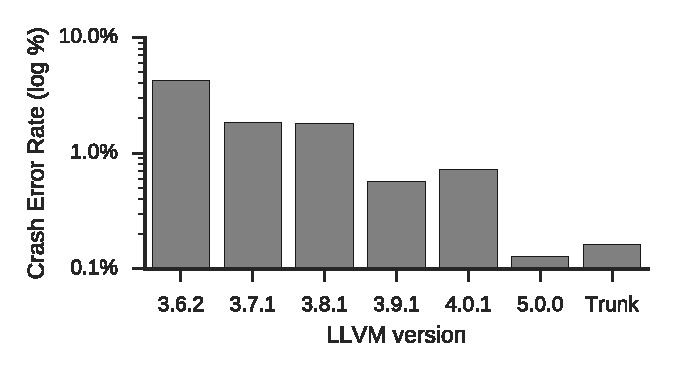
\includegraphics[width=.85\columnwidth]{img/clang-crashes}%
  \caption[Crash rate of the Clang front-end]{%
    Crash rate of the Clang front-end of every LLVM release in the past 24 months compiling 75k DeepSmith kernels.%
  }%
  \label{fig:clang-clash-rate}
\end{figure}

\begin{table}
  \centering %
  \begin{tabular}{r|ccccccc}
  \toprule
  {} & 3.6.2 & 3.7.1 & 3.8.1 & 3.9.1 & 4.0.1 & 5.0.0 & Trunk \\
  \midrule
  Assertion 1 & 2962 & 1327 & 1332 & 414 & 523 & 83 & 97 \\
  Assertion 2 & & 1 & 1 & & & &       \\
  Assertion 3 & & & & & & & 1 \\
  Assertion 4 & & & & & & & 2 \\
  Assertion 5 & 147 & & & & & &       \\
  Assertion 6 & 1 & & & & & &       \\
  Assertion 7 & & & & 1 & 1 & &       \\
  Unreachable & 86 & 42 & 14 & 14 & 18 & 13 & 21 \\
  \bottomrule
\end{tabular}

  \caption[Number of DeepSmith programs which trigger errors]{%
    The number of DeepSmith programs which trigger distinct Clang front-end assertions, and the number of programs which trigger unreachables.%
  }
  \label{tab:clang-crash-rate}
\end{table}

The results emphasise that compiler validation is a moving target. Every change and feature addition has the potential to introduce regressions or new failure cases. Since LLVM will not release unless their compiler passes their own extensive test suites, this also reinforces the case for compiler fuzzing. DeepSmith provides an effective means for the generation of such fuzzers, at a fraction of the cost of existing techniques.


\subsection{Extensibility of Language Model}
\label{subsec:deepsmith-solidity-extensibility}

\begin{table}
  \centering %
  \caption{%
    The number of DeepSmith programs that trigger Solidity compiler crashes in 12 hours of testing.%
  }
  \begin{tabular}{|rc|ccc|}
    \hline
    \rowcolor{gray!50}
    \textbf{Compiler} & $\pm$ & \textbf{Silent Crashes} & \textbf{Assertion 1} & \textbf{Assertion 2}\\
    \multirow{ 2}{*}{solc}    & $-$ & 204 & 1 & \\
    & $+$ & 204 & 1 & \\
    \rowcolor{gray!25}
    & $-$ & 3628 & 1 & 1\\
    \rowcolor{gray!25}
    \multirow{ -2}{*}{solc-js} & $+$ & 908 & 1 & 1\\
    \hline
  \end{tabular}
  \label{tab:preliminary-solidity-results}
\end{table}


A large portion of the DeepSmith architecture is language-agnostic, requiring only a corpus, encoder, and harness for each new language. This potentially significantly lowers the barrier-to-entry compared with prior grammar-based fuzzers. This section reports on initial results in extending DeepSmith to the Solidity programming language. Solidity is the smart contract programming language of the Ethereum blockchain. At less than four years old, it lacks much of the tooling of more established programming languages. Yet, it is an important candidate for rigorous testing, as exploitable bugs may undermine the integrity of the blockchain and lead to fraudulent transactions.


\subsubsection{Testing Methodology}

The same methodology was applied to train the program generator as for OpenCL. A corpus of Solidity contracts was assembled from GitHub, recursively inlining imported modules where possible. The same tokeniser was used as for OpenCL, only changing the list of language keywords and builtins. Code style was enforced using clang-format. The model is trained in the same manner as OpenCL. No modification to either the language model or generator code was required. A simple compile-only test harness is used to drive the generated Solidity contracts.


\subsubsection{Initial Results}

The generator and harness loop was run for 12 hours on four testbeds: the Solidity reference compiler \texttt{solc} with optimisations on or off, and \texttt{solc-js}, which is an Emscripten compiled version of the \texttt{solc} compiler. Table~\ref{tab:preliminary-solidity-results} summarises the results. Numerous cases were found where the compiler silently crashes, and two distinct compiler assertions. The first is caused by missing error handling of language features (this issue is known to the developers). The source of the second assertion is the JavaScript runtime and is triggered only in the Emscripten version, suggesting an error in the automatic translation from LLVM to JavaScript.

Extending DeepSmith to a second programming required an additional 150 lines of code (18 lines for the generator and encoder, the remainder for the test harness) and took about a day. Given the re-usability of the core DeepSmith components, there is a diminishing cost with the addition of each new language. For example, the OpenCL encoder and re-writer, implemented using LLVM, could be adapted to C with minimal changes. Given the low-cost of extensibility, these preliminary results indicate the utility of the approach for simplifying test case generation.


\section{Summary}
\label{sec:deepsmith-conclusion}

This chapter presents a novel framework for compiler fuzzing. By posing the generation of random programs as an unsupervised machine learning problem, the cost and human effort required to engineer a compiler fuzzer are drastically lowered. This aims to address the \emph{adoption challenge} of machine learning (Section~\ref{subsec:challenge-adoption}). Large parts of the stack are programming language-agnostic, requiring only a corpus of example programs, an encoder, and a test harness to target a new language.

The approach is demonstrated by targeting the challenging many-core domain of OpenCL. The implementation, DeepSmith, has uncovered dozens of bugs in both commercial and open-source OpenCL compilers. DeepSmith exposed bugs in parts of the compiler where current approaches have not, for example in missing error handling. A preliminary exploration of the extensibility of this approach to other languages has been performed. DeepSmith test cases are small, two orders of magnitude shorter than the state-of-the-art, and easily interpretable.
